\documentclass[aspectratio=169,11pt]{beamer}

% Compile with pdfLaTeX on Overleaf or TeX Live.
\usepackage[utf8]{inputenc}
\usepackage[T1]{fontenc}
\usepackage[english]{babel}
\usepackage{lmodern}
\usepackage{graphicx}
% Find images next to main.tex (Overleaf) or in report/ (local project).
\graphicspath{{./}{report/}}

\definecolor{DeepBlue}{HTML}{003B70}
\definecolor{AccentRed}{HTML}{C8102E}
\definecolor{BodyInk}{HTML}{202B36}
\definecolor{SoftBlue}{HTML}{EAF1F7}
\setbeamercolor{normal text}{fg=BodyInk,bg=white}
\setbeamercolor{structure}{fg=DeepBlue}
\setbeamercolor{frametitle}{fg=white,bg=DeepBlue}
\setbeamercolor{title}{fg=DeepBlue}
\setbeamercolor{block title}{fg=white,bg=DeepBlue}
\setbeamercolor{block body}{fg=BodyInk,bg=SoftBlue}
\setbeamerfont{frametitle}{series=\bfseries,size=\Large}
\setbeamertemplate{navigation symbols}{}
\setbeamertemplate{itemize item}{\color{AccentRed}\textbullet}
\setbeamertemplate{itemize subitem}{\color{AccentRed}--}
\setbeamertemplate{footline}[frame number]
\setbeamersize{text margin left=9mm,text margin right=9mm}
\setlength{\parskip}{0.4em}

% Place background.png next to main.tex. Use a white background if it is missing.
\IfFileExists{background.png}{%
  \usebackgroundtemplate{%
    \includegraphics[width=\paperwidth,height=\paperheight]{background.png}%
  }%
}{}

\title{ESP32 SMART HOME}
\subtitle{System Overview and Demonstration}
\author{Project Team}
\date{}

\begin{document}

\begin{frame}[plain]
  \vfill
  {\large\color{AccentRed}\bfseries PROJECT DEMONSTRATION}\par
  \vspace{0.35cm}
  {\Huge\color{DeepBlue}\bfseries ESP32 SMART HOME}\par
  \vspace{0.25cm}
  {\color{AccentRed}\rule{0.16\textwidth}{2pt}}\par
  \vspace{0.25cm}
  {\large System Overview and Demonstration}\par
  \vspace{0.5cm}
  {\small Project Team}
  \vfill
\end{frame}

\begin{frame}{Presentation Outline}
  \vfill
  {\Large\bfseries\color{AccentRed} 01}\quad {\large\bfseries System Overview and Progress}\par
  \vspace{0.7cm}
  {\Large\bfseries\color{AccentRed} 02}\quad {\large\bfseries Hardware Demo}\par
  \vspace{0.7cm}
  {\Large\bfseries\color{AccentRed} 03}\quad {\large\bfseries App Demo}
  \vfill
\end{frame}

% PART 1: System overview and work completed by the team.
\begin{frame}{1. Problem and Objectives}
  \begin{columns}[T,onlytextwidth]
    \begin{column}{0.48\textwidth}
      \textbf{Problem}
      \begin{itemize}
        \item Users need to control and monitor home devices from a phone.
        \item Devices and the app need to exchange data over a shared network.
      \end{itemize}
    \end{column}
    \begin{column}{0.48\textwidth}
      \textbf{Team Objectives}
      \begin{itemize}
        \item Build a control system using ESP32.
        \item Use MQTT to exchange commands, device states and sensor events.
        \item Test each subsystem before full integration.
      \end{itemize}
    \end{column}
  \end{columns}
\end{frame}

\begin{frame}{1. System Architecture}
  \centering
  \vfill
  % Overall system: app, message queue, ESP32, sensors and actuators.
  % Editable source: report/architecture.mmd.
  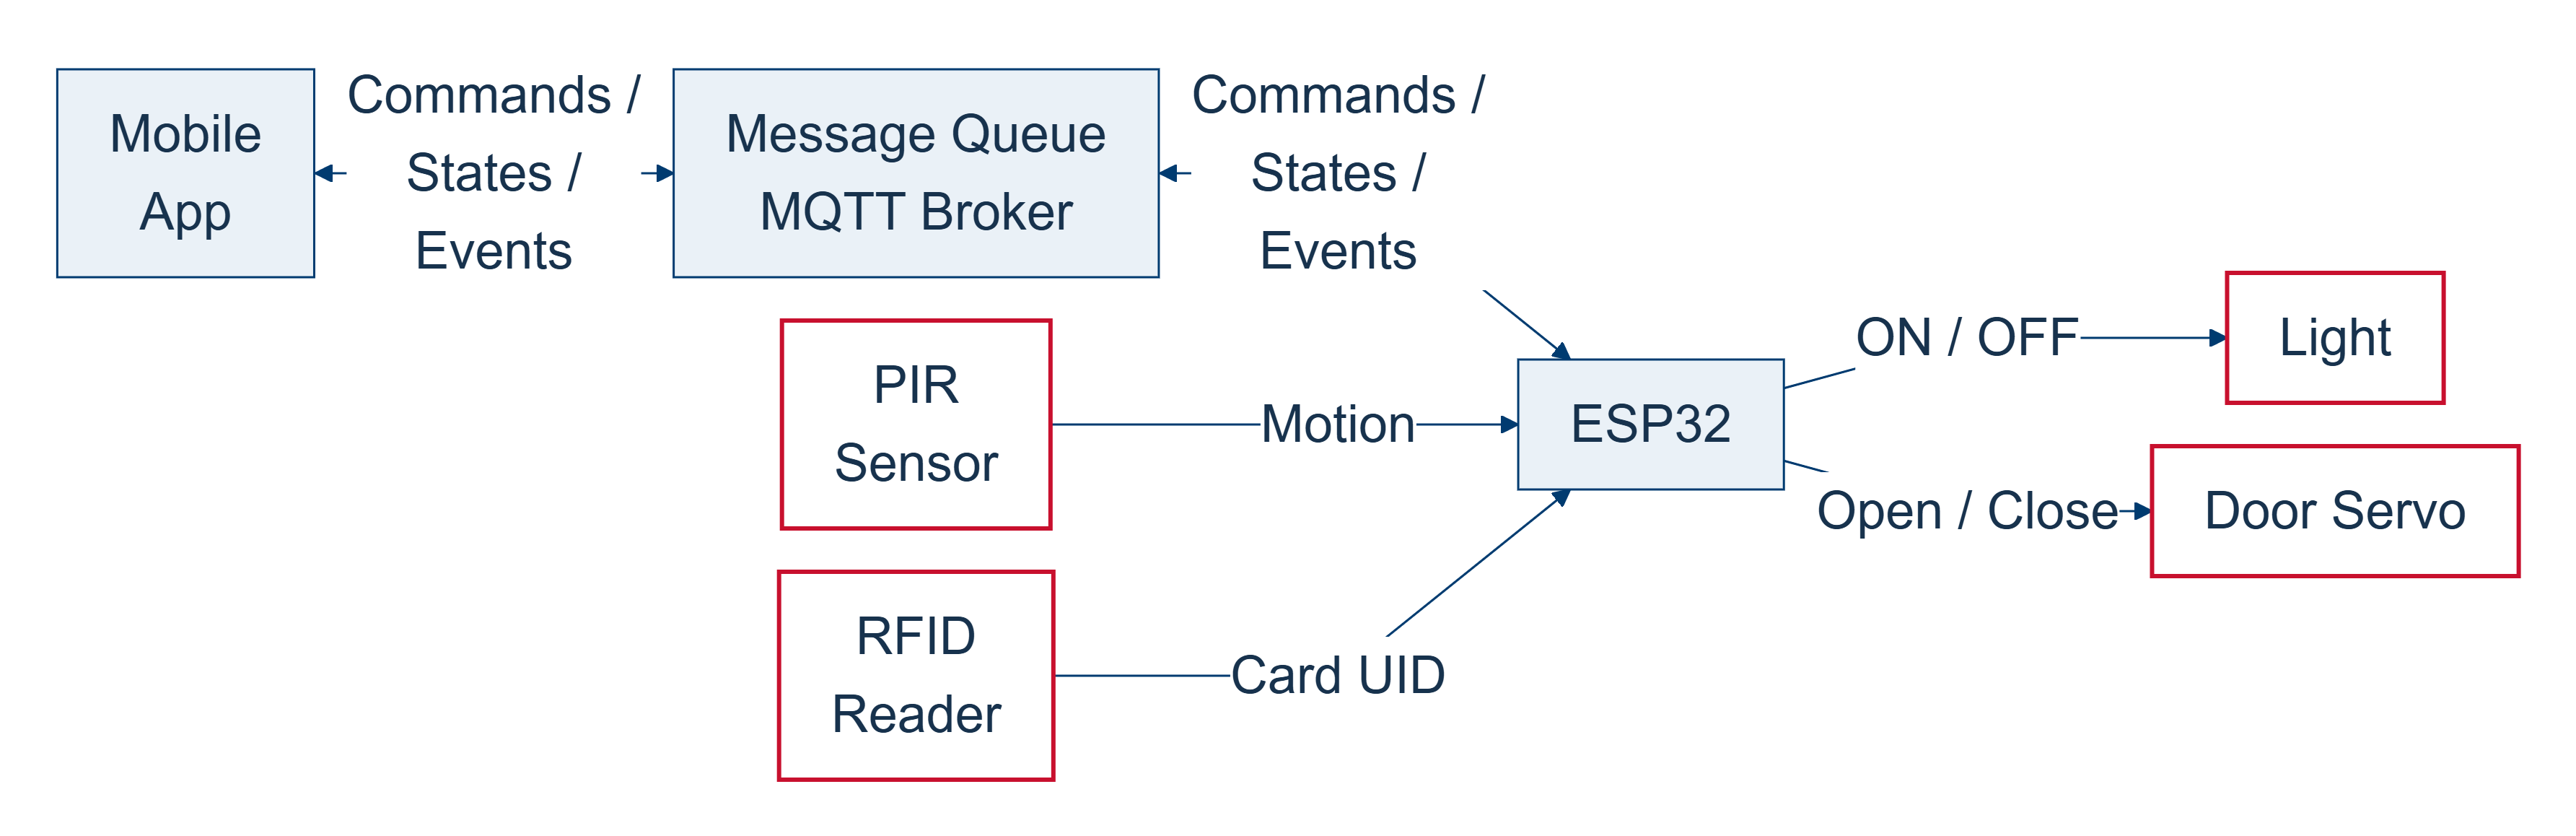
\includegraphics[width=\textwidth,height=0.72\textheight,keepaspectratio]{architecture.png}
  \vfill
  {\small Target system architecture with bidirectional MQTT communication.}
\end{frame}

\begin{frame}{1. System Components}
  \begin{itemize}
    \setlength{\itemsep}{0.65em}
    \item \textbf{Firmware:} Wi-Fi and MQTT connections, command handling.
    \item \textbf{Hardware:} light and door control, PIR sensing and RFID reading.
    \item \textbf{Broker:} EMQX message routing with Docker Compose configuration.
    \item \textbf{User Interface:} dashboard prototype and mobile app skeleton.
    \item \textbf{Integration:} shared topics, payloads and communication tests.
  \end{itemize}
  \vspace{0.3cm}
  {\small Hardware and interface development continues on separate branches.}
\end{frame}

\begin{frame}{1. Hardware Integration Branch Features}
  \begin{columns}[T,onlytextwidth]
    \begin{column}{0.47\textwidth}
      {\large\bfseries\color{DeepBlue} Light and Motion}\par
      \vspace{0.3cm}
      Receives ON/OFF commands over MQTT. PIR motion detection can also trigger the light.
    \end{column}
    \begin{column}{0.47\textwidth}
      {\large\bfseries\color{DeepBlue} Door and RFID}\par
      \vspace{0.3cm}
      A servo opens and closes the door. A card on the allowlist triggers a door-open request.
    \end{column}
  \end{columns}
  \vspace{0.7cm}
  \textcolor{AccentRed}{\bfseries Feedback}\quad Device states and access events are published over MQTT.
  \vspace{0.45cm}

  {\small These features exist in the integration branch code and need testing on real hardware.}
\end{frame}

\begin{frame}{1. MQTT Communication}
  \centering
  {\large\bfseries Example: Turn On the Light and Receive Its State}\par
  \vfill
  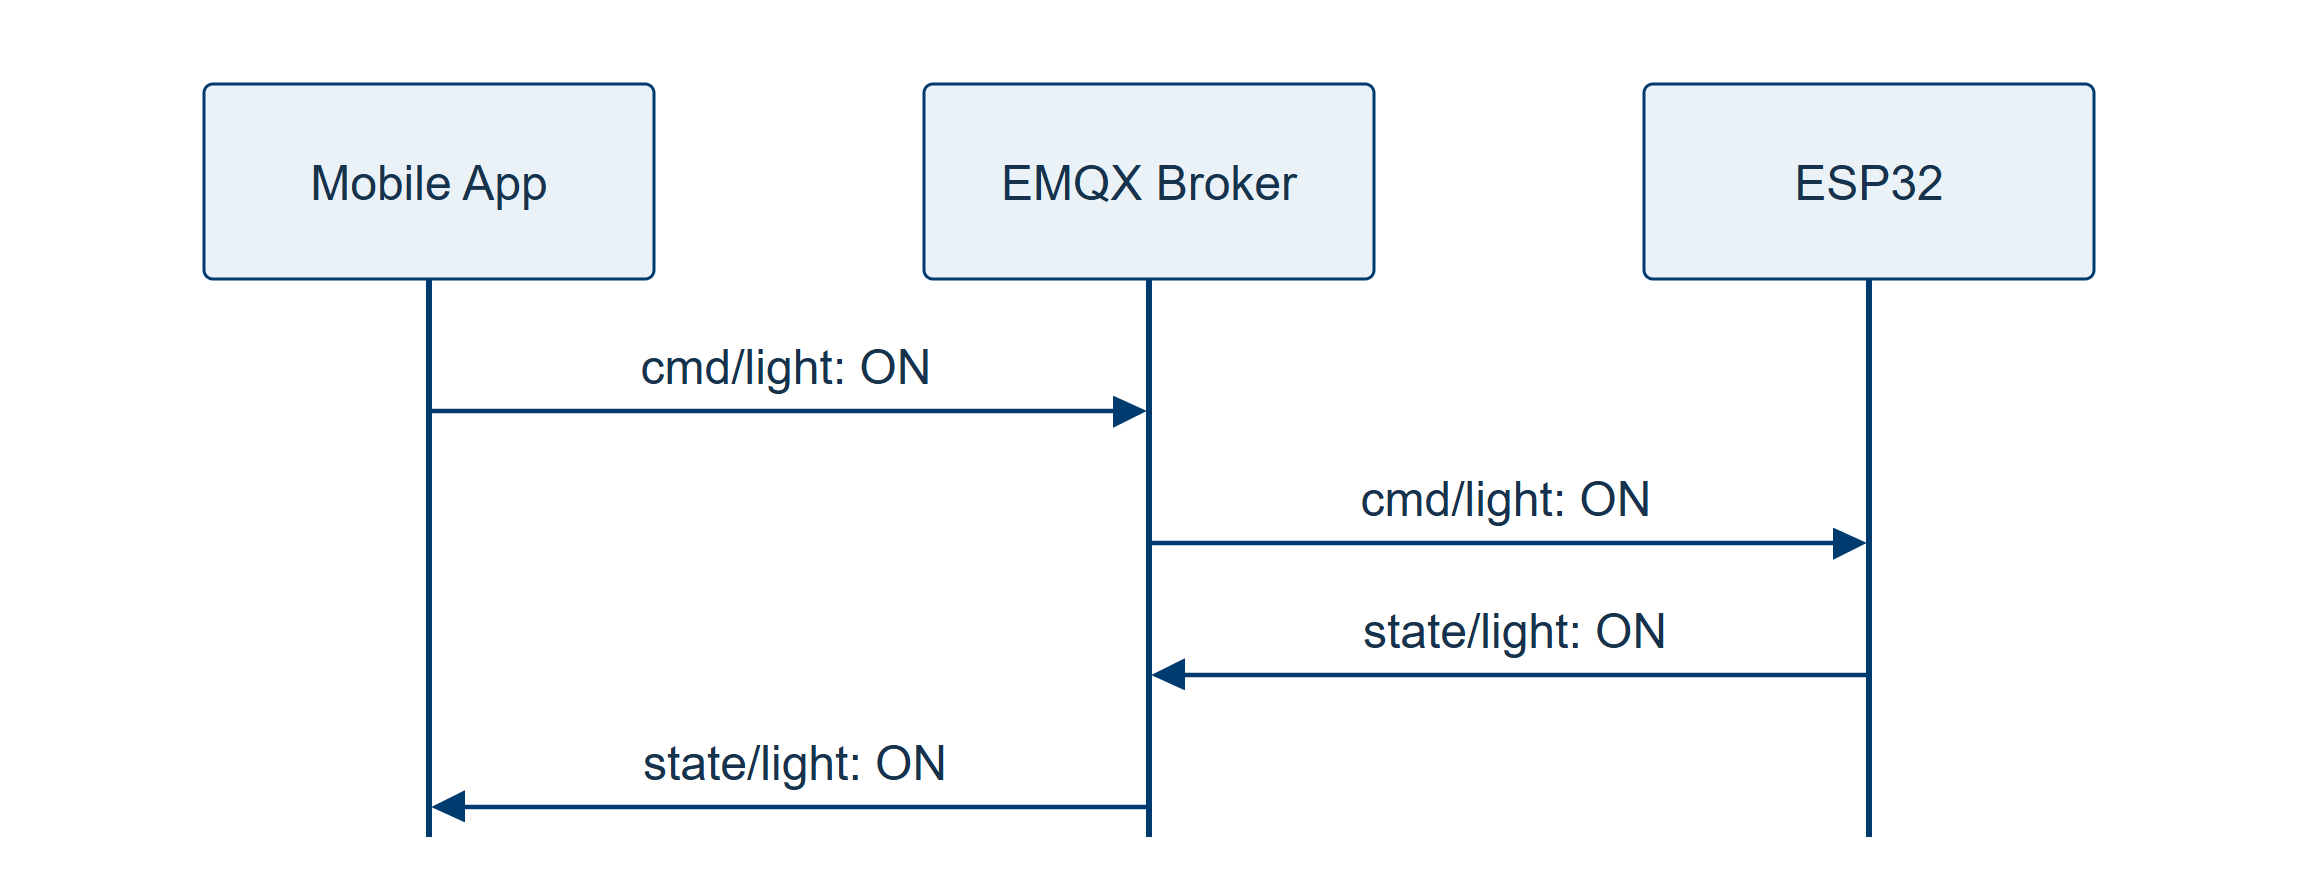
\includegraphics[width=0.88\textwidth,height=0.57\textheight,keepaspectratio]{mqtt-flow.png}
  \vfill
  {\small All topics start with \texttt{smarthome/}. State feedback needs integration testing.}
\end{frame}

\begin{frame}{1. Work Completed}
  \begin{columns}[T,onlytextwidth]
    \begin{column}{0.52\textwidth}
      {\large\bfseries\color{DeepBlue} Implemented}\par
      \begin{itemize}
        \item Firmware, broker and MQTT contract.
        \item Light, door, PIR and RFID code on the hardware integration branch.
        \item Web interface prototype.
      \end{itemize}
    \end{column}
    \begin{column}{0.43\textwidth}
      {\large\bfseries\color{DeepBlue} Tested}\par
      \vspace{0.25cm}
      {\Huge\bfseries\color{AccentRed} 4/4}\par
      The local broker correctly forwards all four light and door commands.

      {\small ESP32 command reception is recorded based on the team's confirmation.}
    \end{column}
  \end{columns}
  \vspace{0.4cm}
  {\small Broker test results do not confirm full system operation.}
\end{frame}

\begin{frame}{1. Next Integration Tasks}
  \begin{itemize}
    \setlength{\itemsep}{0.7em}
    \item Merge the hardware and interface branches into the shared system.
    \item Align MQTT topics and payloads between the app and ESP32.
    \item Verify command and state flows on real hardware.
    \item Test reconnection and collect acceptance test evidence.
  \end{itemize}
  \vspace{0.5cm}
  {\small Current documentation does not yet include full system integration test evidence.}
\end{frame}

% PART 2: Add hardware demo photos, videos and content here.
\begin{frame}{2. Hardware Demo}
  \centering
  \vfill
  {\Large\color{DeepBlue}\bfseries Hardware Demo}

  \vspace{0.45cm}
  {\normalsize Add demo photos, videos or content here.}
  \vfill
\end{frame}

% PART 3: Add app demo screenshots, videos and content here.
\begin{frame}{3. App Demo}
  \centering
  \vfill
  {\Large\color{DeepBlue}\bfseries App Demo}

  \vspace{0.45cm}
  {\normalsize Add demo screenshots, videos or content here.}
  \vfill
\end{frame}

\begin{frame}[plain]
  \centering
  \vfill
  {\Huge\bfseries\color{DeepBlue} Thank You!}

  \vspace{0.5cm}
  {\large Questions and Discussion}
  \vfill
\end{frame}

\end{document}
